\chapter{Технологический раздел}

В этом разделе будут рассмотрены средства разработки программного продукта и детали его реализации.

\section{Средства реализации}

Для реализации программного продукта был выбран язык программирования С++ \cite{cpp}. Этот язык является компилируемым, что дает преимущество в скорости в сравнении с интерпретируемыми языками программирования. С++ поддерживает различные механизмы объектно-ориентированного программирования такие как инкапсуляция, наследование и полиморфизм. Эта парадигма сочетается с задачей отображения объектов реального мира, так как каждый объект можно задать с помощью отдельного класса с соответствующим набором полей и методов \cite{oop}.

Для реализации интерфейса приложения был выбран фреймворк Qt \cite{qt}. Данный выбор обусловлен тем, что он содержит все базовые классы, которые требуются для интерфейса приложения, а также позволяет выгружать содержимое сцены в файл.

Для создания модульных тестов был выбран фреймворк GoogleTests \cite{gtest}. Данный выбор обусловлен тем, что он включает в себя определения основных классов и макросов, которые используются для создания модульных тестов.

Для автоматической сборки и тестирования работы приложения использовалась платформа gitlab.

\section{Формат входных и выходных данных}

На вход программа принимает 2 параметра:
\begin{itemize}
	\item Имя конфигурационного файла, описывающего объекты сцены.
	\item Флаг, отвечающий за отключение пользовательского интерфейса. Если установлен флаг -no-gui, то сцена считывается из конфигурационного файла и сохраняется в файл, после чего программа завершает свою работу.
\end{itemize}

Результатом работы программы является сцена, которая отображается в окне пользовательского интерфейса или сохраняется в файл.

\subsection{Формат файла-описателя модели}
Пример файла описателя планеты представлен на листинге \ref{lst:planet.txt}

\listingfile{planet.txt}{}{Пример файла описателя планеты}{}
Первые три значения в файле - координаты центра объекта, относительно которого заданы все остальные точки. После идет число точек, из которых состоит объект и их координаты. Дальше указано число поверхностей и их свойства. Первые три числа в строке с поверхностью - индексы точек, из которых она состоит, после указывается номер цвета в таблице цветов и коэффициент диффузного отражения поверхности. После указано число узлов, по которым строится анимация объекта. Каждый узел состоит из координат и момента времени, когда центр модели находится в них.

\subsection{Формат файла-описателя источника света}
Пример файла описателя источника света представлен на листинге \ref{lst:source.txt}

\listingfile{source.txt}{}{Пример файла-описателя источника света}{}

Здесь первое число отвечает за интенсивность источника (от 0 до 255). Дальше идет описание геометрических свойств аналогично файлу-описателю планеты.

\subsection{Формат файла-описателя камеры}
Пример файла описателя камеры представлен на листинге \ref{lst:camera.txt}

\listingfile{camera.txt}{}{Пример файла-описателя камеры}{}

Первые три числа - координаты задающие положение наблюдателя. На следующей строке задаются углы поворота камеры относительно осей x, y и z соответственно.

\subsection{Формат файла описателя сцены}
Пример файла описателя камеры представлен на листинге \ref{lst:scene.yaml}

\listingfile{scene.yaml}{}{Пример файла-описателя сцены}{}

Источник света, камера и таблица цветов создаются из конфигурационных файлов, которые расположены по базовым путям $./data/light\_source.txt$, $./data/camera.txt$ и $./data/color\_table.txt$ соответственно.

В поле $planets$ идет перечисление файлов-описателей планет, из которых состоит система. Группа атрибутов $time$ описывает время в системе. Если атрибут $is\_video$ равен $true$, то создается несколько  фотографий сцены со временем в системе от $time\_start$ до $time\_finish$ с шагом  $time\_step$ не включительно. Иначе создается только одно изображение со временем из атрибута $cur\_time$. Группа атрибутов $scaling$ отвечает за масштаб изображения. $kx$ за масштаб по оси х, $ky$ ~---~ y. Группа $scene_params$ отвечает за размеры изображения сцены. Атрибут $width$ содержит значение ширины, а $height$ ~---~ высоты. Группа атрибутов $camera\_rotation$ отвечает за углы поворота камеры. Атрибуты $xangle$, $yangle$ и $zangle$ содержат значения относительно осей x, y и z соответственно.

\section{Реализация основных модулей системы}

Реализация алгоритма z-буфера представлена на листинге \ref{lst:zbuffer.cpp}

\listingfile{zbuffer.cpp}{c}{z-буфер}{}

\section{Тестирование системы}
В рамках тестирования программы были выделены следующие случаи
\begin{itemize}
	\item Все объекты находятся на одной линии и перекрывают друг друга
	\item Один объект находится в тени другого
	\item Повороты камеры
	\item Изменение масштаба
\end{itemize}

Результаты тестов приведены на рисунках \ref{img:test_one_line} - \ref{img:test_scaling}
\begin{center}
	\begin{figure}[H]
		\centering
		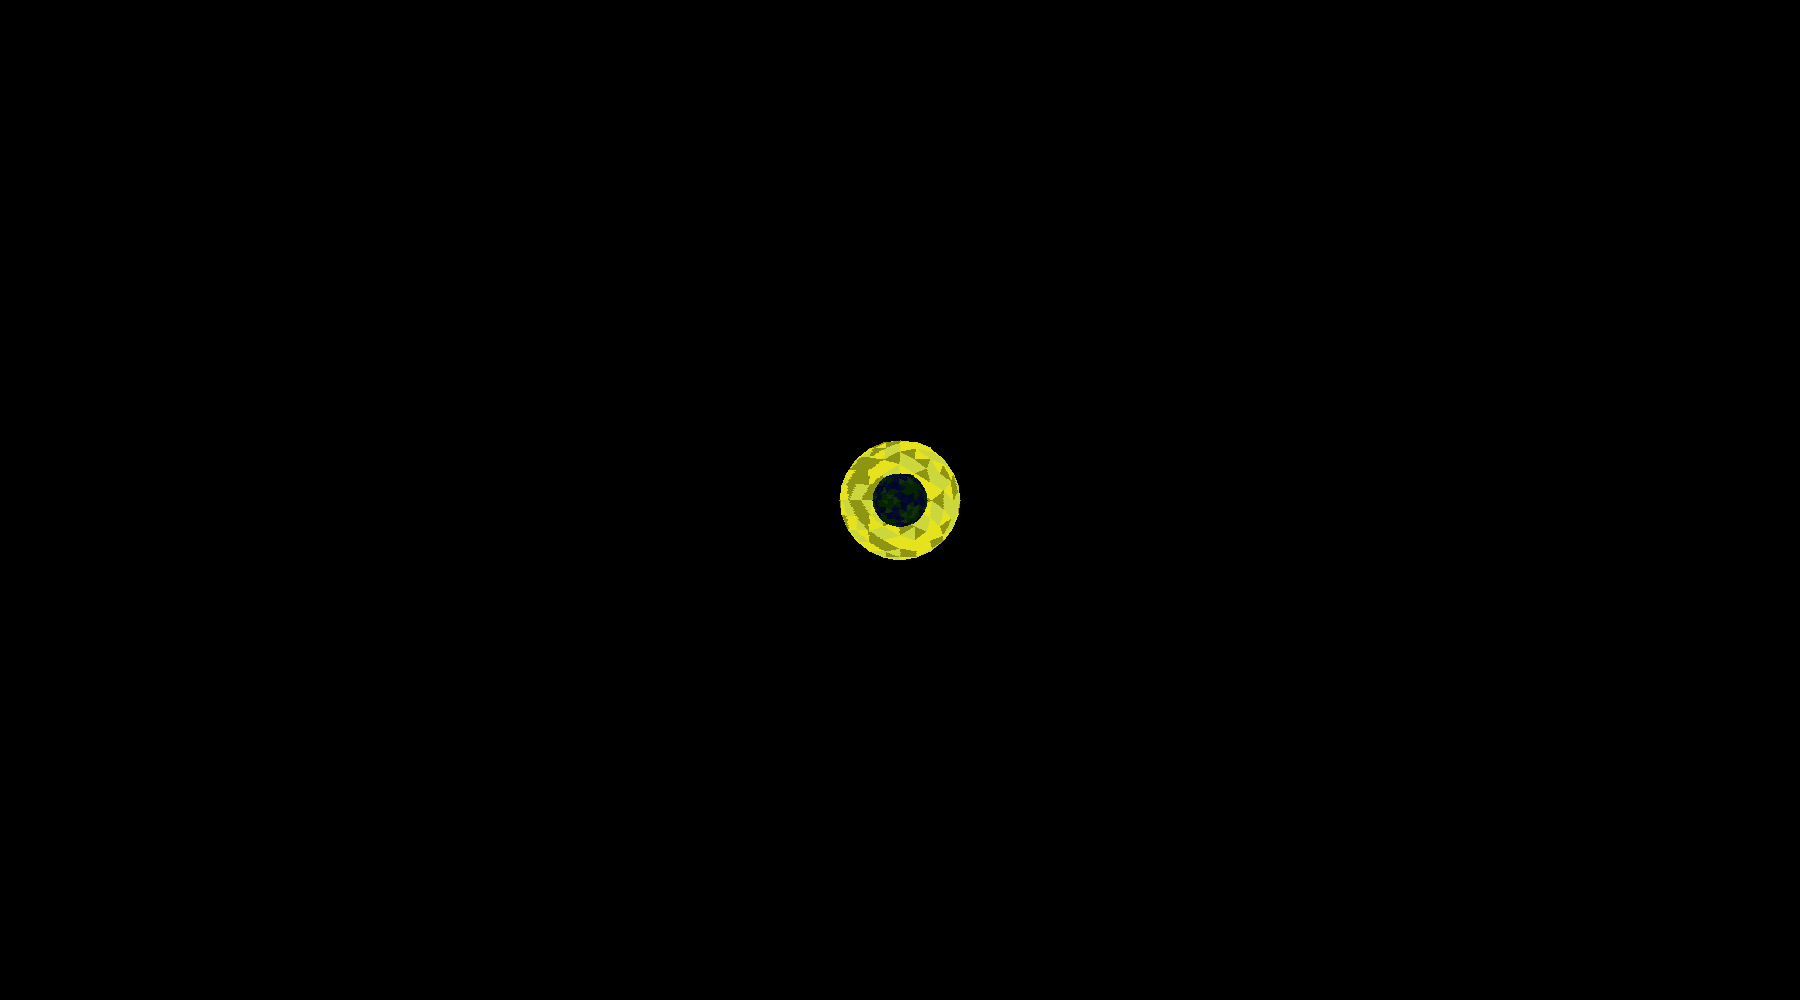
\includegraphics[scale=0.3]{inc/img/one_line.png}
		\caption{Объекты находятся на одной линии}
		\label{img:test_one_line}
	\end{figure}
\end{center}

\begin{center}
	\begin{figure}[H]
		\centering
		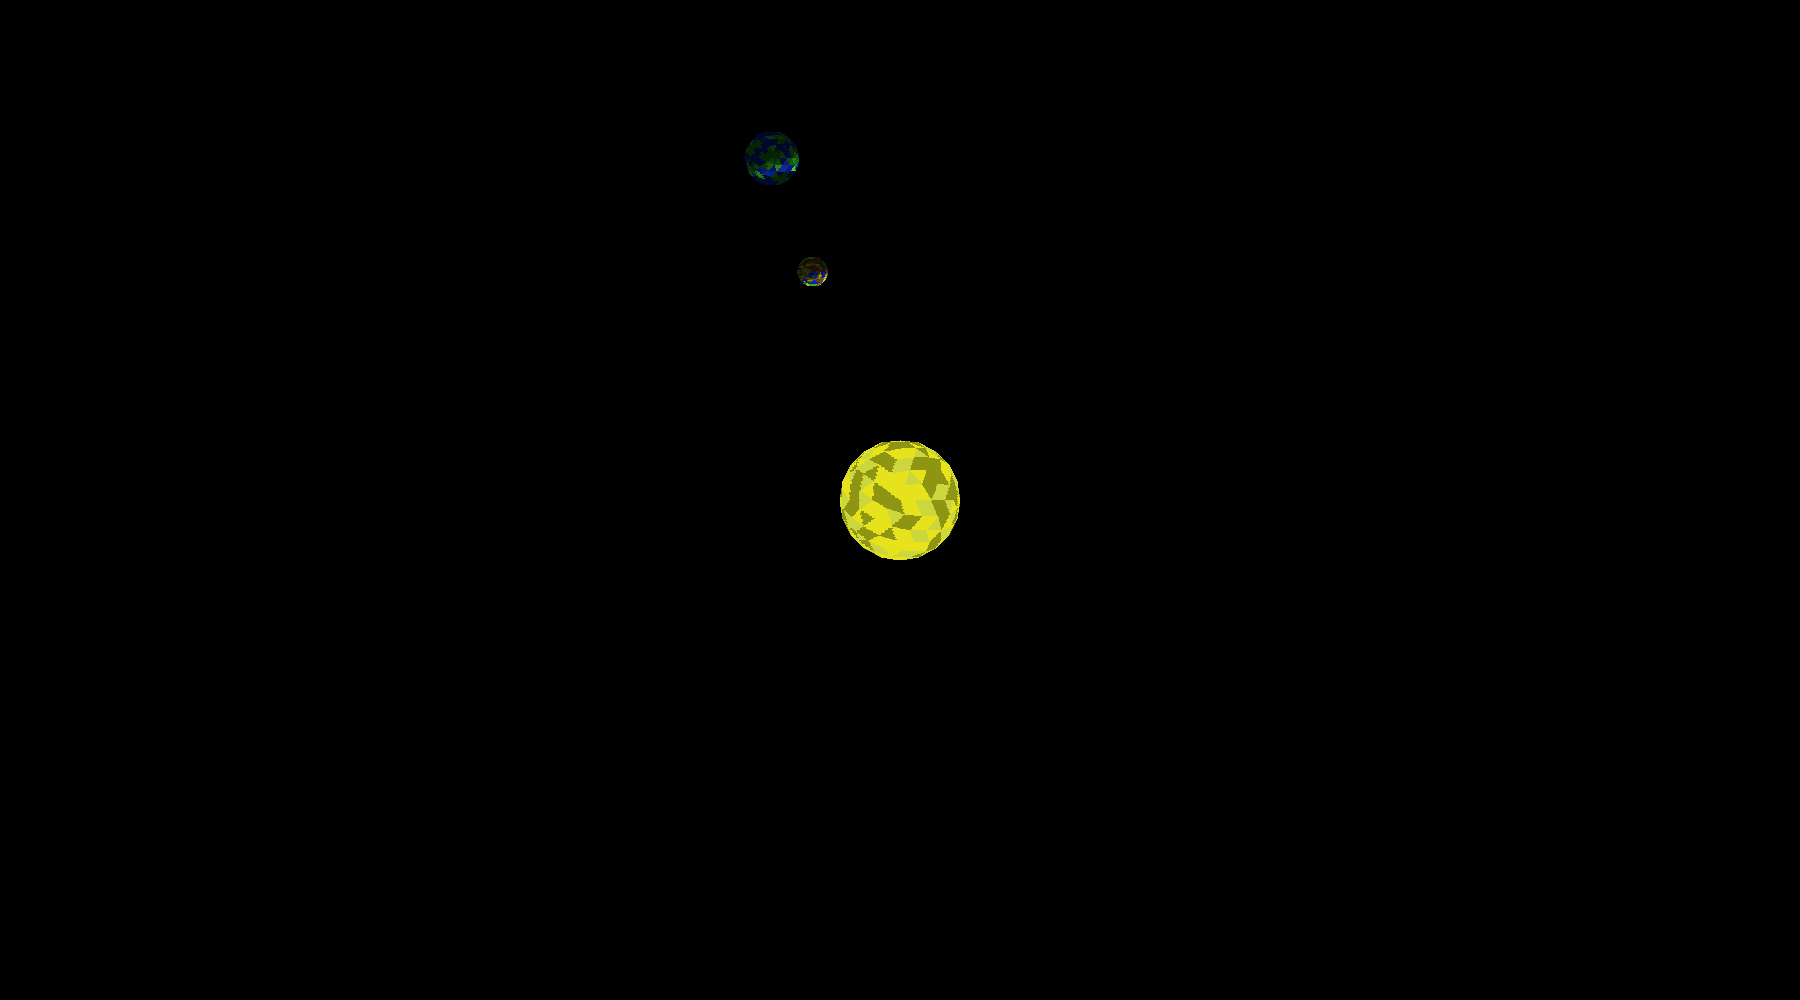
\includegraphics[scale=0.3]{inc/img/shadow.png}
		\caption{Один объект находится в тени другого}
		\label{img:test_shadow}
	\end{figure}
\end{center}

\begin{center}
	\begin{figure}[H]
		\centering
		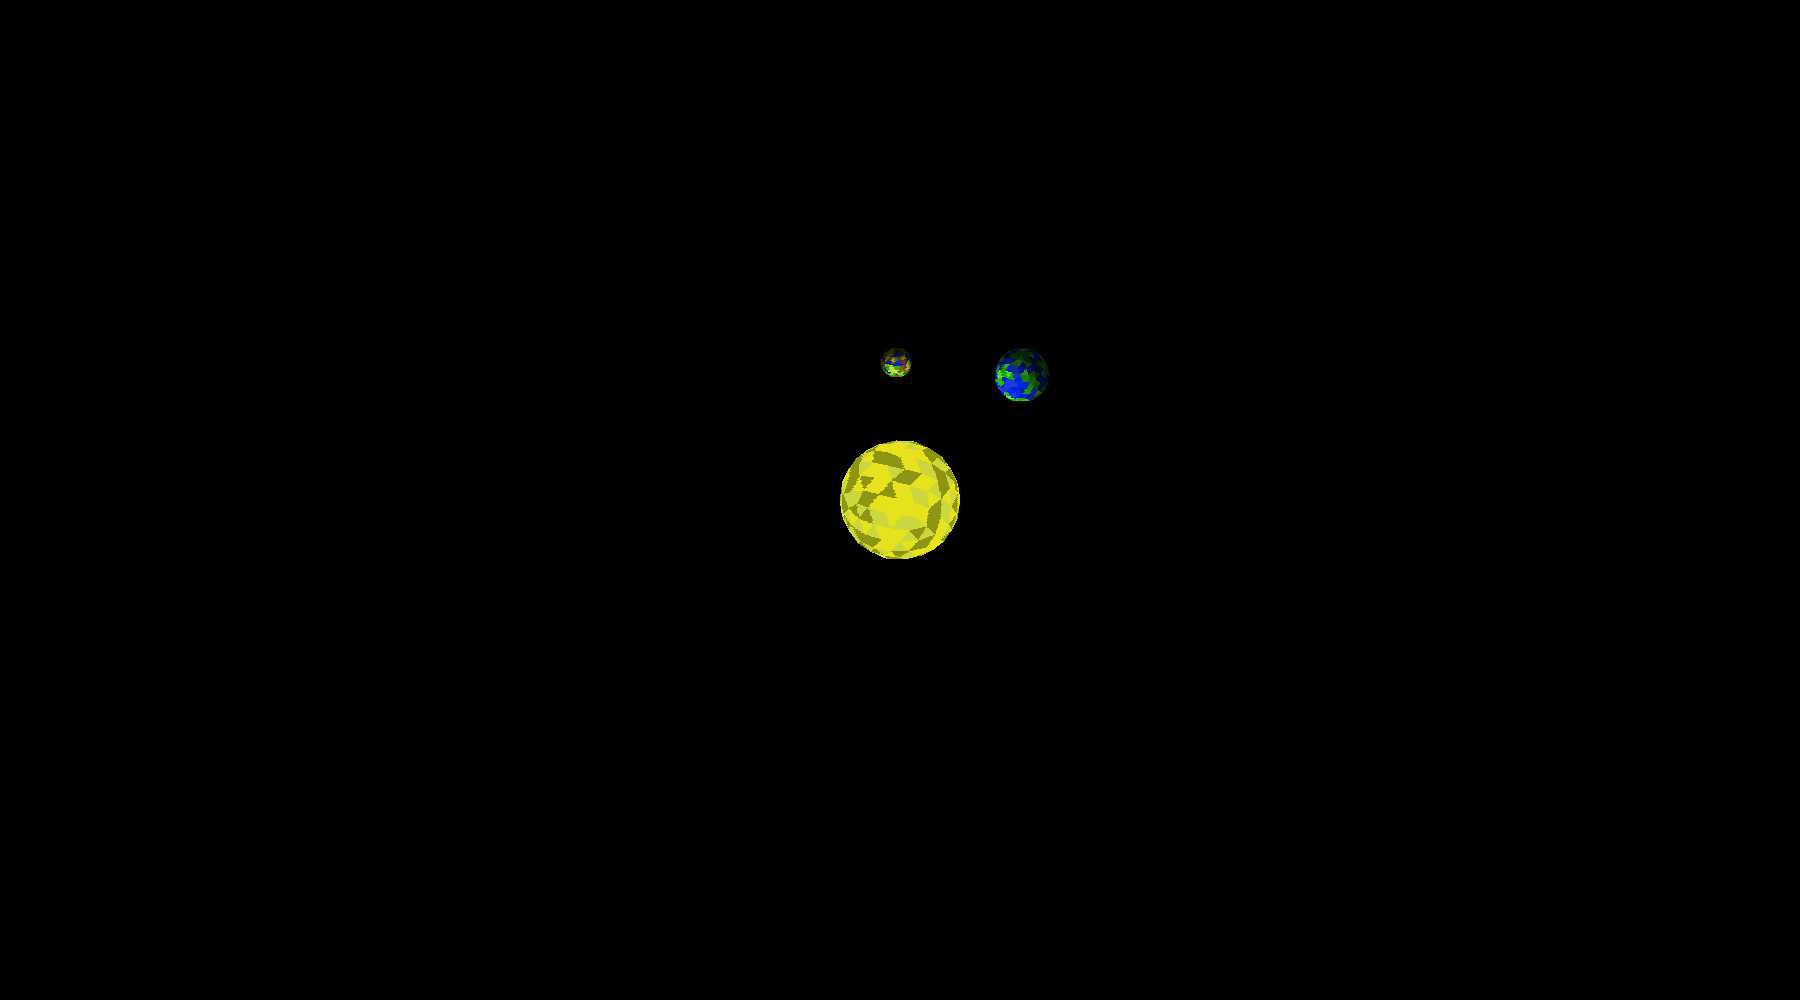
\includegraphics[scale=0.3]{inc/img/xrotation.png}
		\caption{Поворот вокруг оси x}
		\label{img:test_xrotation}
	\end{figure}
\end{center}

\begin{center}
	\begin{figure}[H]
		\centering
		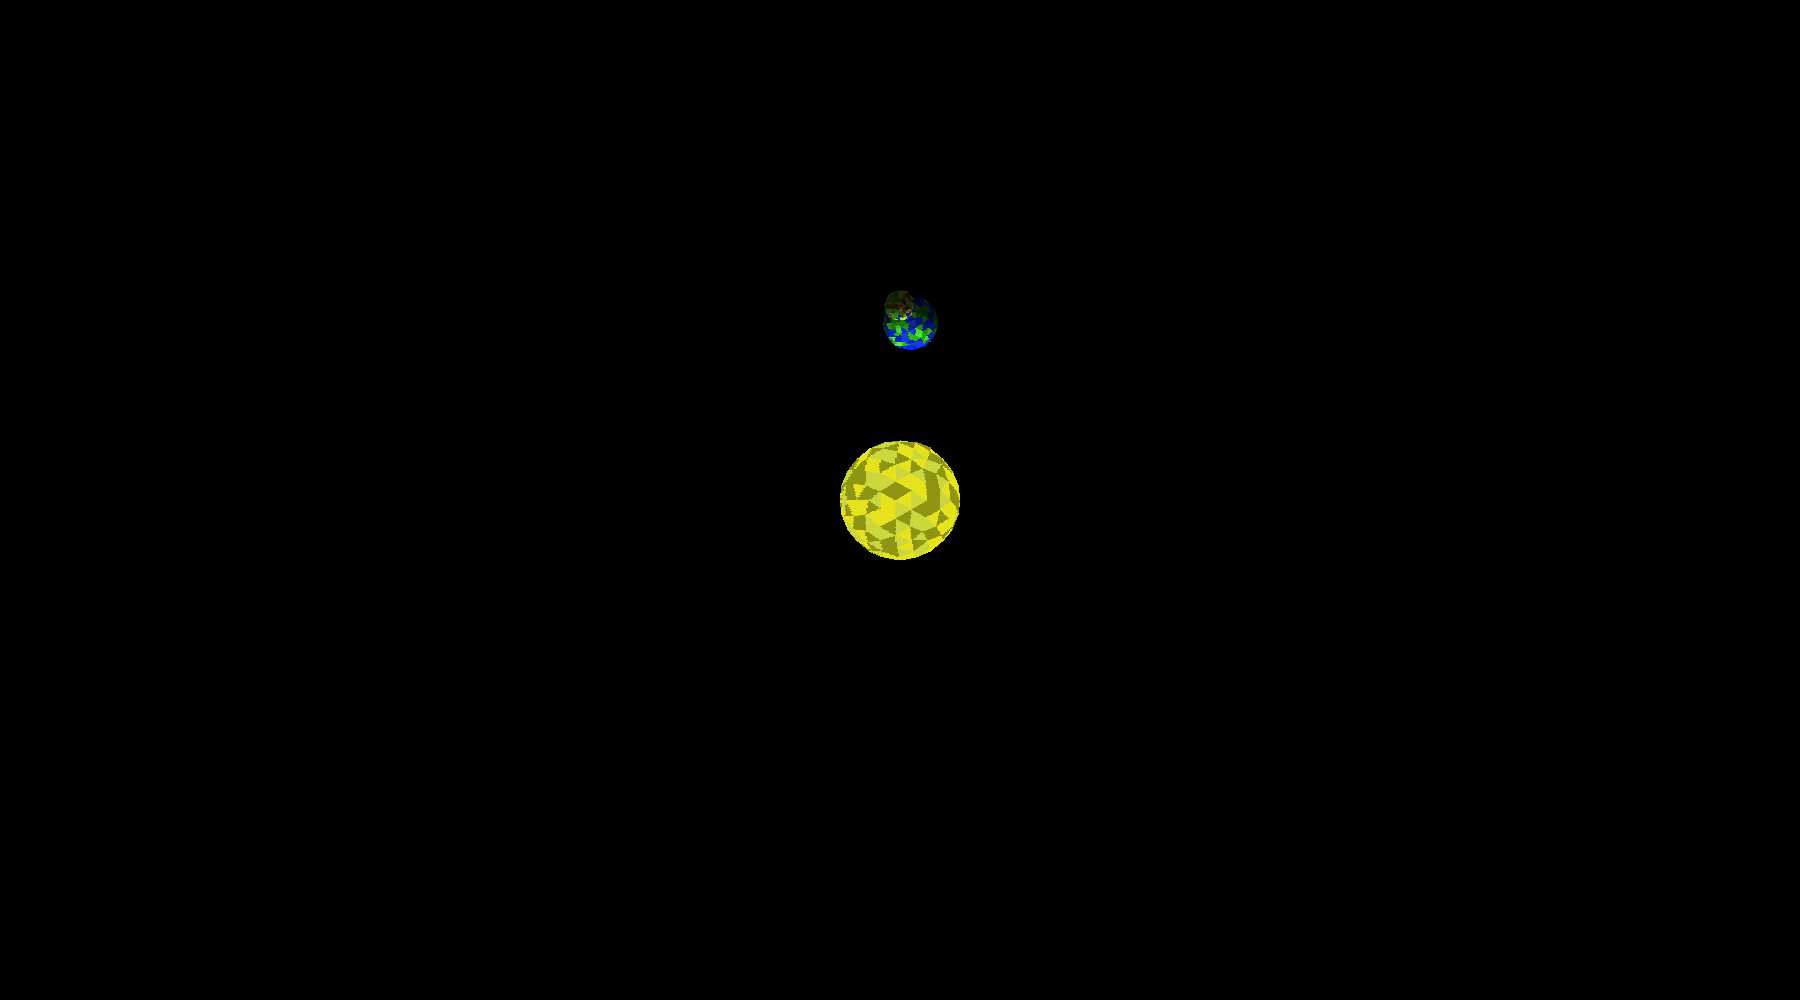
\includegraphics[scale=0.3]{inc/img/yrotation.png}
		\caption{Поворот вокруг оси y}
		\label{img:test_yrotation}
	\end{figure}
\end{center}

\begin{center}
	\begin{figure}[H]
		\centering
		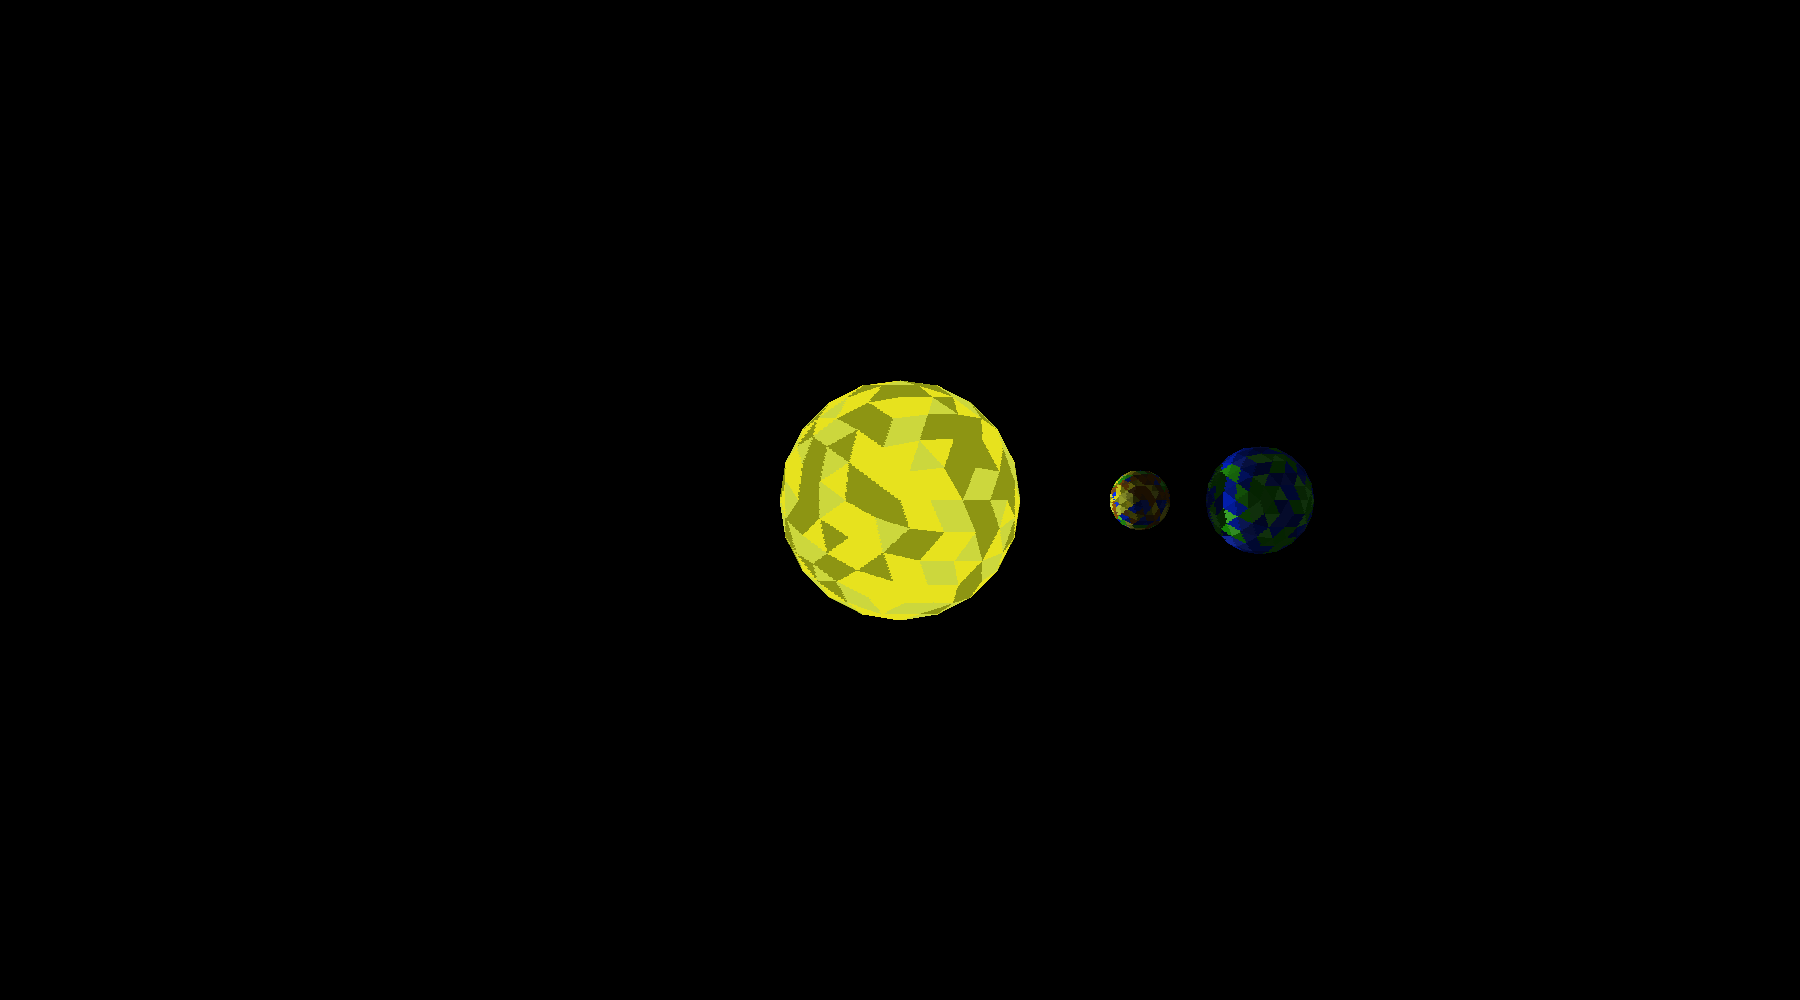
\includegraphics[scale=0.3]{inc/img/scaling.png}
		\caption{Изменение масштаба}
		\label{img:test_scaling}
	\end{figure}
\end{center}

Все тесты успешно пройдены.

\section{Вывод}
В данном разделе были выбраны средства реализации программного продукта, определены форматы входных и выходных данных, а также был реализован и протестирован алгоритм z-буфера.